\documentclass[a4paper, 12pt]{article}
\usepackage[T1,T2A]{fontenc}
\usepackage[utf8x]{inputenc}
\usepackage{graphicx}
\usepackage[labelsep=period]{caption}
\graphicspath{{pictures/}}
\usepackage[english,russian]{babel}
\usepackage{amsmath}
\usepackage{color,graphicx,ulem,cmap}
\usepackage{subfigure}
\title{основная часть}
\author{я}
\begin{document}


\begin{figure}[ht!]  
\vspace{-4ex} \centering \subfigure[]{
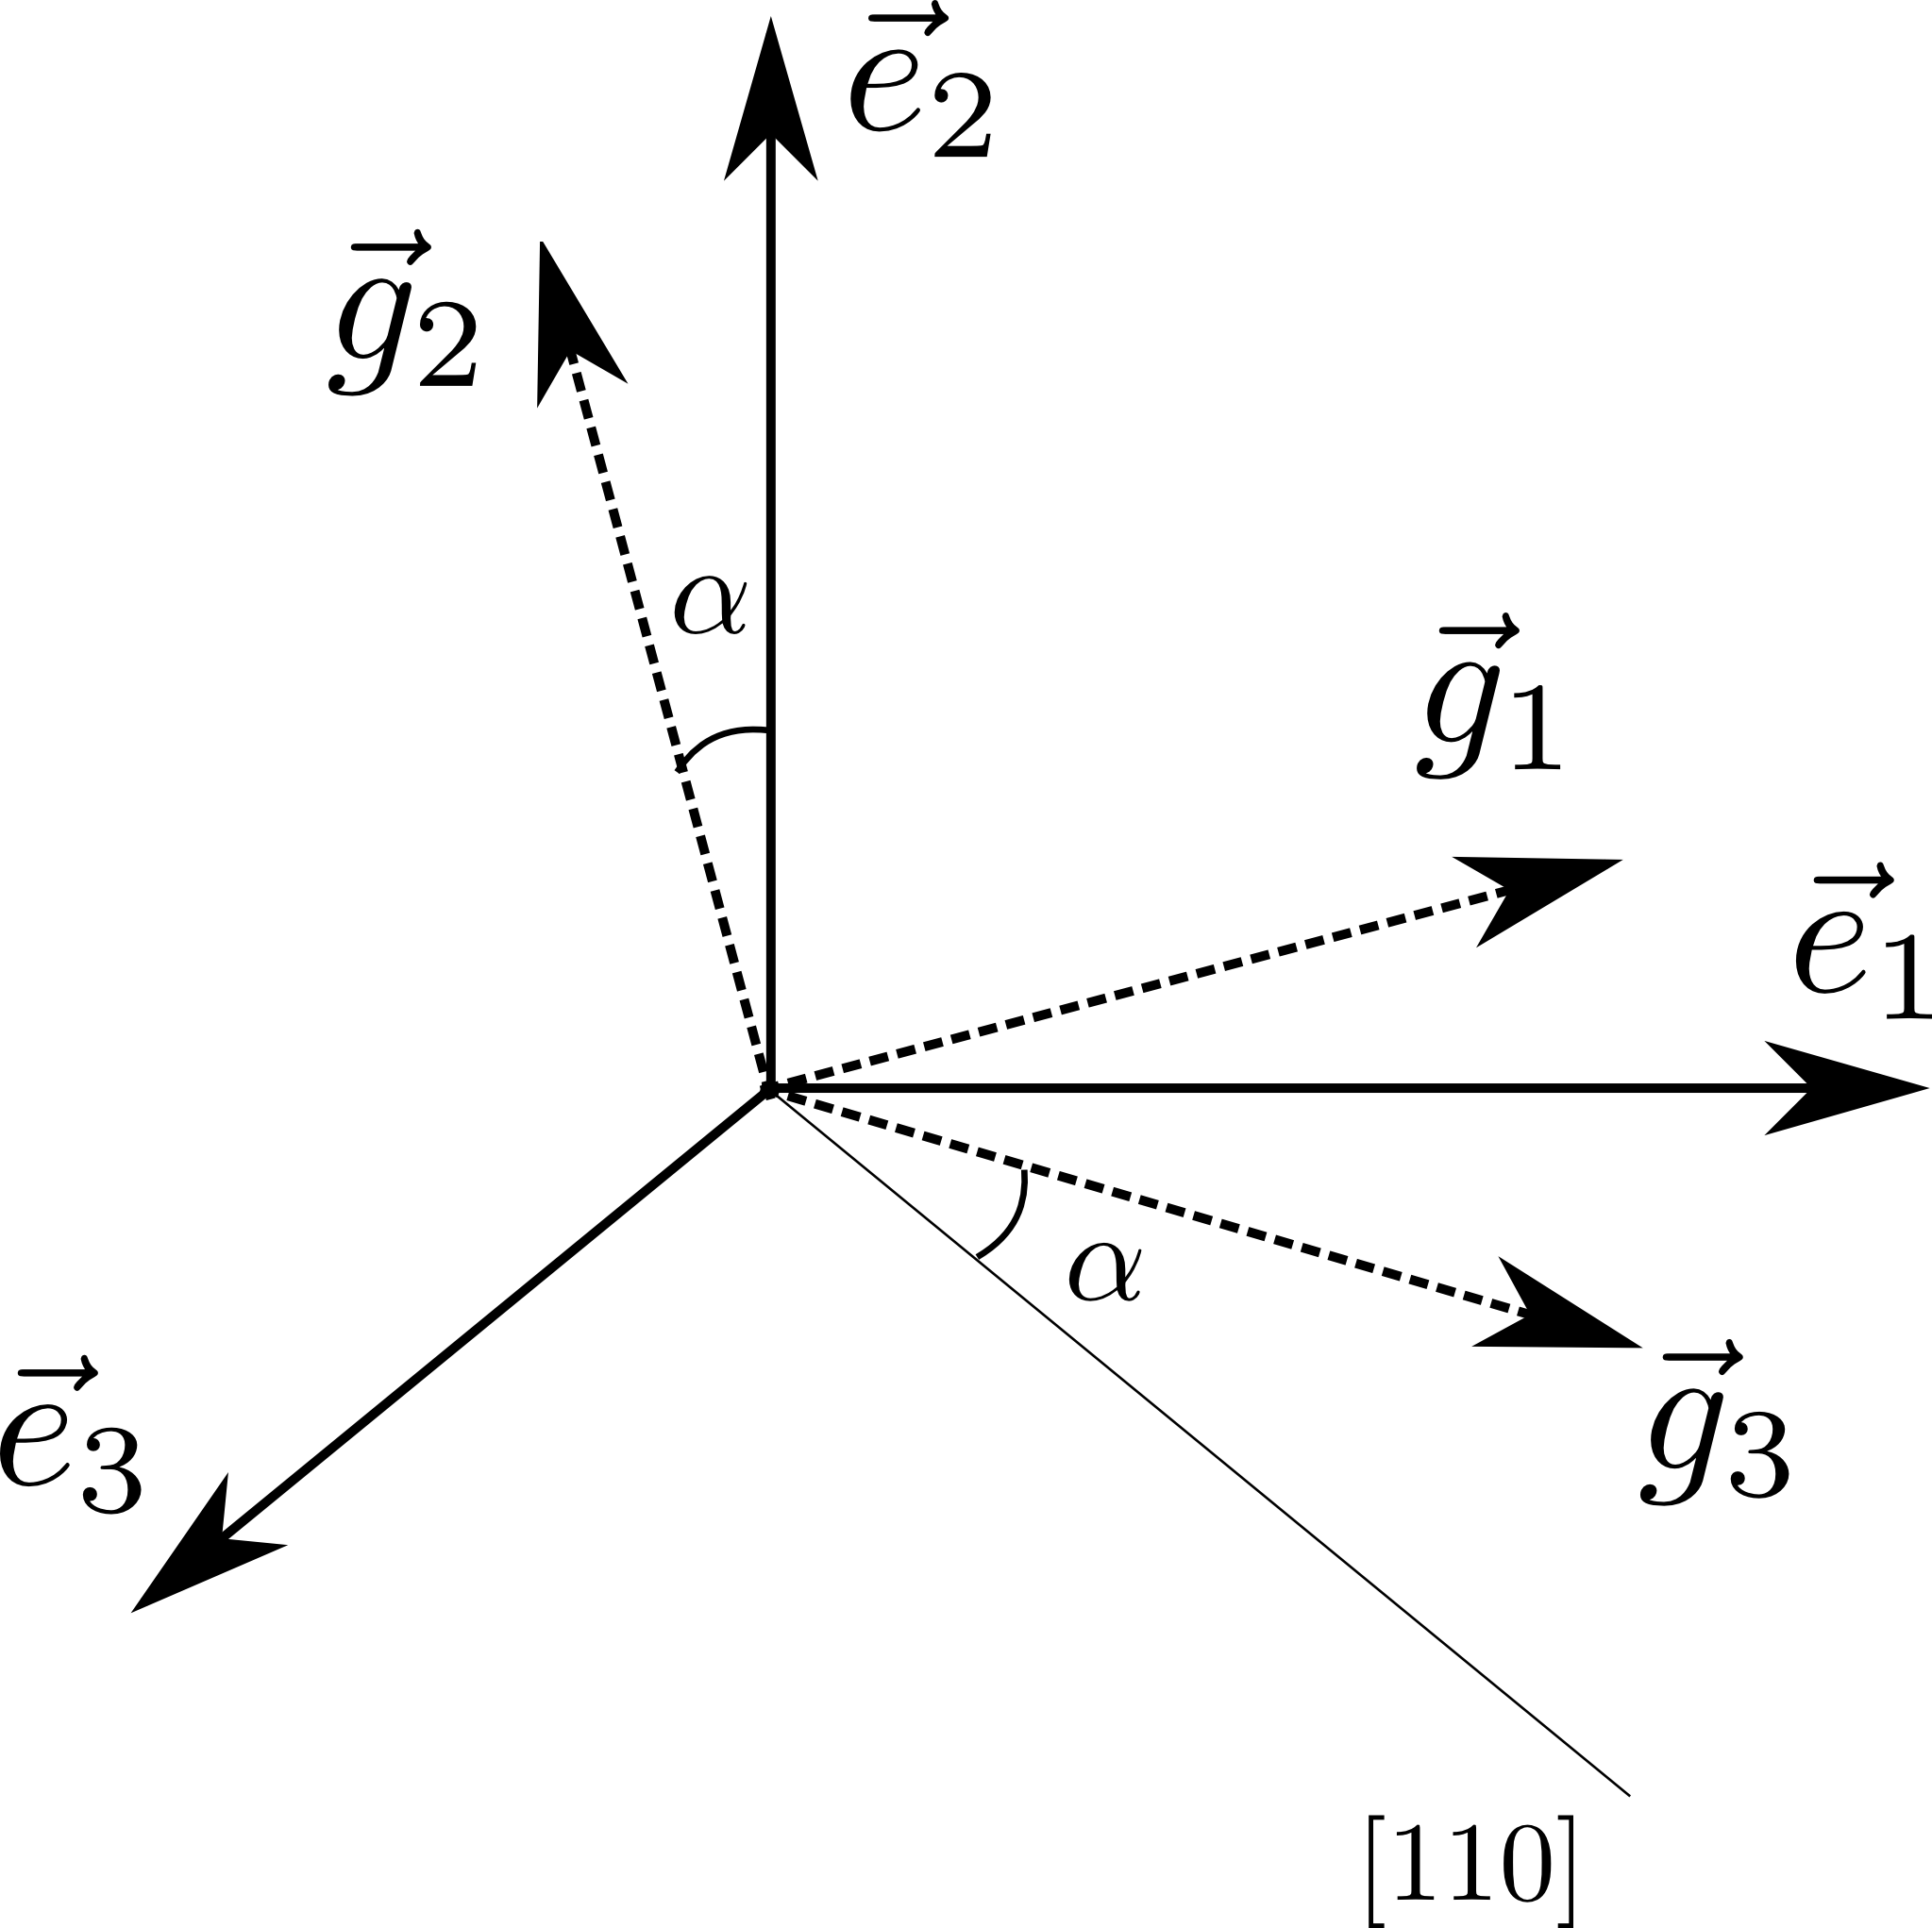
\includegraphics[width=0.25\linewidth]{1.png} \label{fig:aaa} }  
\hspace{4ex}
\subfigure[]{
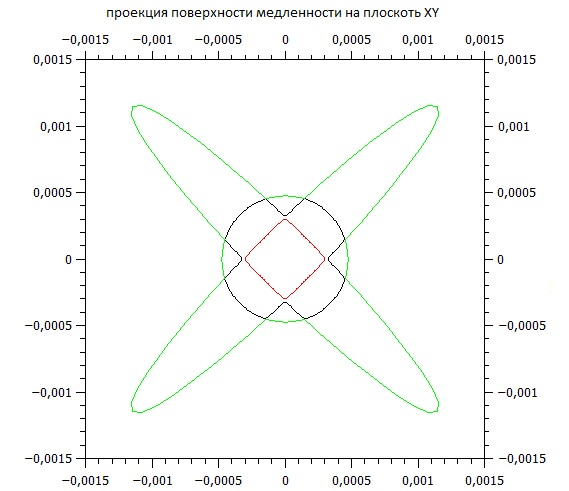
\includegraphics[width=0.25\linewidth]{2.png} \label{fig:bbb} }
\hspace{4ex}
\subfigure[]{ 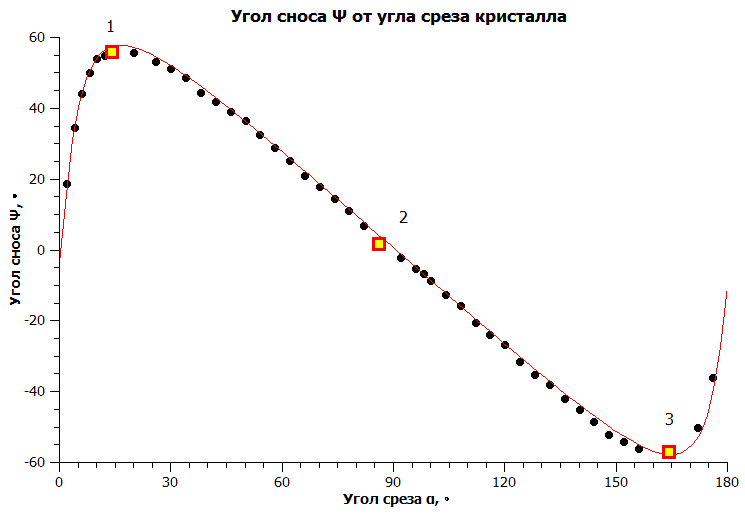
\includegraphics[width=0.24\linewidth]{3.png} \label{fig:ccc} }  
\caption{Coupling cases for the DM models: \subref{fig:aaa} decoupled case; \subref{fig:bbb} coupling between the closest neighbours; \subref{fig:ccc} coupling between the closest neighbour and diagonally adjacent actuators.} \label{fig:threeDMcases}
\end{figure}

\end{document}
